%!TEX root = ../BPlusTree-report.tex
\section{Background}
\label{sec:Background}
% Notes:
% What is a bplustree:
%   - Inherently imperative data structure
%   - Suboptimal implementation
%     - Running time of optimal implementation
%     - Running time of our implementation
%       - Mention how one could make it optimal.
%       - A tree in a tree in a tree, dawg
%     - Running time out of scope

\subsection{Gallina}
Gallina is a purely functional specification language\todo{ref}, which is used by the Coq interactive proof assistant. It is very lean, and does not include non-functional data structures, such as arrays\todo{ref}. 

\subsection{B+ tree}
The B+ tree is a n-ary, self-balancing, tree data structure\todo{ref}, similar to a B-tree\todo{ref}. It is composed of a root, nodes, and leaves. The root may be a leaf or a node. Nodes hold pairs of keys and pointers, $(k, p)$. $p$ points to either a node or leaf that holds the values over $k$, but below the key of the next pair. Leaves hold pairs of keys and values, $(k, v)$. In this project keys are always natural numbers, while values can have any type, denoted by $X$. 

\begin{figure}
 \centering
   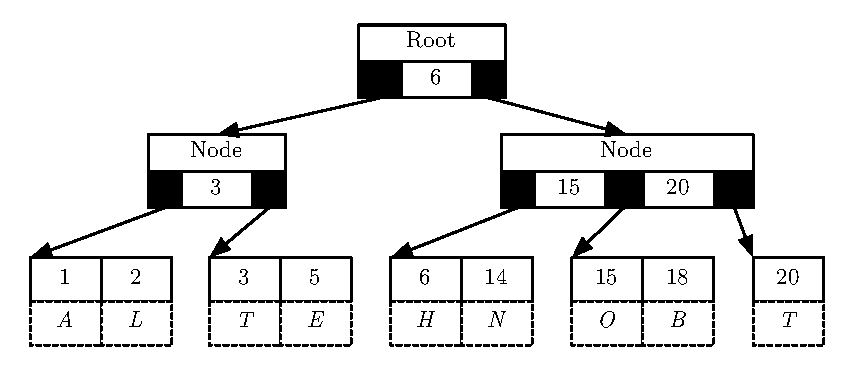
\includegraphics[width=90mm]{diagrams/BPlusTree.pdf}
 \caption{An example of a B+ tree with $b=2$. The bottom row contains leaves, with values, in this case characters, in the dashed boxes.}
 \label{fig:bplustree}
\end{figure}

For a given B+ tree, a branching factor $b$ determines the capacity of nodes and leaves\todo{ref}. A node must have at least $b/2$ children, and at most $b$. A leaf must have between $b/2$ and $b$ values. This rule is relaxed for the root node, which must have between 2 and $b$ children.

\subsubsection{Implementation}
In our implementation, a node is a list of $(k, p)$ pairs, and a leaf is a list of $(k, v)$ pairs, through which we perform a linear search to find the correct value. Since Gallina does not support arrays, the only way to get lookups faster than $O(n)$ is through a tree structure, such as a B+ tree. This would add a large degree of complexity to our proofs, and since running time is not an objective of this project, it has been deemed out of scope.